\documentclass[a4paper,11pt]{article}
\usepackage{fancyhdr}
\usepackage{hyperref}
\usepackage{rotating}

\usepackage{enumitem}
\setlist[description]{font={\normalfont\slshape}}

\usepackage{import}
\subimport{../latex/}{setup_report.tex}


\fancyhf{}
\lhead{Andreas Stöckel}
\rhead{SYDE 750 Project Report}
\cfoot{\thepage}


\title{Learning Probability Distributions for Statistical Inference \\[1em] \Large SYDE 750 Project Report}
\author{Andreas Stöckel}
\date{April 20, 2017}

\addbibresource{../bibliography/bibliography.bib}

\begin{document}

\maketitle

\begin{abstract}
Psychological research by Griffiths et al. suggests that humans are capable of near-optimal Bayesian inference for high-level cognitive tasks. In this report, I describe and analyze a simple neural architecture capable of learning a prior probability distribution from empirical measures and performing statistical inference. The proposed network architecture represents probability distributions as a sum of weighted, near-orthogonal, and non-negative basis functions. Weights are learned with the Prescribed Error Sensitivity (PES) rule. Inference is performed by changing the underlying function space followed by gradient descent. I compare the model to human data collected on the Lifespan Inference Task proposed by Griffiths et al.~and discuss strengths and weaknesses of the model.
\end{abstract}

% Structure of the report
% =======================
%
% - Introduction
%   - Motivation
%     - Cognition as Bayesian inference
%     - Bayesian inference for high level cognitive tasks <== build a model of this!
%   - Structure of the report
% - Mathematical Model of Lifetime Inference
% - Proposed network architecture
%   - Mathematical model
%   - Step1: System description
%     - Identify the relevant neurobiological properties
%     - Specify the representations as variables
%     - Provide a functional description
%   - Step 2: Design specification
%     - Specify the range, precision, and signal-to-noise ratio for each variable
%     - Specify the temporal and dynamic characteristics for each variable
%   - Step 3: Implementation
%     - Specify the decoding rules
%     - Determine which parts of the model are to be simulated to which degrees of detail
%     - Perform numerical experiments using resulting simulation

\pagebreak

\pagestyle{fancy}
\tableofcontents

\pagebreak

\section{Introduction}
\label{sec:introduction}

In their 2006 research article \emph{Optimal Predictions in Everyday Cognition}, Griffiths and Tennenbaum conduct a set of psychological experiments in which they analyze statistical inference performed by humans in the context of high-level cognitive tasks. They argue that low-level cognition such as sensorimotor learning is known to approximate optimal Bayesian inference (see \cite{kording2004bayesian} for an example), whereas high-level, everyday judgments are often described as \enquote{error-prone heuristics that are insensitive to prior probabilities} \cite{griffiths2006optimal}. To contrast this line of thought, the authors present a set of high-level inference experiments which show that human performance is strikingly close to optimal results derived from ground-truth priors. Goal of this project is to provide a neurobiological model which---just like humans---is able to learn a prior distribution and to solve the so called \enquote{lifespan inference task} presented in the Griffiths and Tennenbaum article in an optimal Bayesian sense.

\subsection{Related work}

Optimal Bayesian inference has been identified as a recurring computational pattern of nervous systems. From a theoretical point of view, some researchers even argue that the whole of cognition can be described as statistical inference of the most likely sensory input, thereby minimizing a measure called \enquote{surprise} or \enquote{free energy} \cite{friston2010free}. Despite this enthusiasm, it is not fully understood how statistical inference is actually implemented in  neurobiological systems. However, a broad range of theories exist, albeit with different notions regarding the kind of and representation over which inference is performed (e.g.~static inference or inference over time, network level computation or single neuron coding scheme, recurrent or feedforward computation \textellipsis). In the following, I try to present the gist of at least some of these theories. Note that the first three theories are explained in \cite{knill2004bayesian}, more detailed descriptions of the others can be found in the indicated works of literature.

\begin{description}
\item[Binary random variables]
The most simple, non-trivial probability distribution $p(x)$ is a distribution over a binary random variable $x \in \{s_1 , s_2\}$. As a neurobiological system, such distributions can be represented with two neuron populations (or even a single population) representing the probability of each possible state. Inference tasks are trivial since all information about the probability distribution is explicit. Evidence for such codes can be found in single cell recordings of the lateral intraparietal cortex (LIP), a part of the parietal lobe, which, among other tasks, is involved in saccadic eye movement \cite{kandel2012principles}.

\item[Convolution codes]
A generalization of the binary random variable model to continuous random variables $x$ can be obtained by sampling $x$ at various locations $x_i$ and representing probabilities $p(x = x_i)$ as individual neuron populations. Individual sample points $p(x = x_i)$ are modeled as Gaussian distributions, allowing to reconstruct a smooth $p(x)$ over the entire domain of $x$. Inference can be performed by multiplying individual sample probability distributions. As always, multiplication can be translated to a simple addition operation when working with logarithmized probabilities.

\item[Gain encoding and probabilistic population codes]
Spike times in cortical neurons can be modeled as a Poisson process. Assume a neuron population, where each neuron possesses a bell-shaped tuning curve corresponding to some stimulus $x$ with different peak locations. Due to the Poisson statistic, the population response $\vec a$ for any given stimulus $x$ contains a relatively high amount of noise, yet resembles a Gaussian distribution with mean $\mu$ and variance $\sigma$. Interestingly, it can be shown that $\sigma$ is inversely proportional to the peak activity in the population and $\mu$ is close to the peak activity. Correspondingly, the population response can be interpreted as a representation of the posterior distribution $p(x \mid \vec a)$. This idea is also referred to as probabilistic population codes, and has been shown to be useful for multisensory integration \cite{ma2006bayesian}.

\item[Neuronal Bayesian inference in time]
Another proposal is the interpretation of the dynamics of individual spiking neurons as Bayesian inference in time \cite{deneve2008bayesian}. In contrast to all other approaches, this theory focuses on single neurons (and not populations of neurons) and individual spikes (and not spike rates). The overall idea is that at a certain time $t$, a single neuron encodes a binary variable $x_t$ which depends on its previous state $x_{t - \Delta t}$. Given a stochastic input, this system can be modeled as a hidden Markov chain, where the current state probabilities are represented as a variable $L$. Surprisingly, $L$ is closely related to the membrane potential of a spiking neuron. In conjunction with spike frequency adaptation (and an additional state variable $G$), the entire system can be interpreted as predicting the expected input and only emitting output spikes (sending information) when the input deviates from the expected value.

\item[Implicit function space representation in the NEF]
In the context of the NEF \cite{eliasmith2003neural}, the activity of a neural ensemble can be seen as representing a function over a certain function space. Naturally, this includes probability density functions, especially conditional probability densities of the form $p(x \mid \vec d)$, where $\vec d$ can be seen as the parameter vector that is actually being represented by the population. A second probability distribution $p(y \mid \vec d)$ can be inferred from an ensemble representing $p(x \mid \vec d)$ with an all-to-all feedforward connection, where the connection weights take $p(x \mid y)$ into account. Interestingly, it possible to select the underlying function space and connection weights in such a way, that no explicit normalization is required \cite{eliasmith2011normalization}. For the task at hand, it seems mildly strange that $\vec d$ is encoded in the neuron activities, and not in synaptic weights, as one would na\"ively expect for prior distributions learned over potentially long timespans.
\end{description}

To varying degrees, the approaches listed above have two shortcomings. First, they are mostly concerned with probability space representation and as such do not provide a simple way to infer a maximum a posteriori or median estimate, which is required for the inference task chosen for this project. Of course, in the context of the NEF, one can always decode the maximum or median from the underlying function space representation. Yet, depending on the function space and the desired accuracy, this may require significant resources. Second, in most of the approaches it is not immediately clear how the prior distribution should be learned \enquote{in vivo}.

The approach I present here draws upon the idea of parameterizing probability distributions over a function space. However, in contrast to the NEF approach discussed above, the basis functions are explicitly computed in connections between neuron ensembles, and parameters are stored in connection weights and not in neural activity. This results in an architecture which partially resembles the convolution coding scheme. The posterior distribution is inferred by exchanging the underlying basis functions, and a median estimate  performed dynamically in time by converging to the optimal state, and not as a feedforward connection.

\subsection{Structure of this report}

The remainder of this report is structured as follows: \cref{sec:lifespan_inference_task} provides a short summary of the psychological experiments performed by Griffiths and Tennenbaum and the mathematical model underlying their analysis. \Cref{sec:pdist_mixture_model} details a mathematical framework for representing, learning and inferring from probability distributions, which I translate into a neurobiological model in \cref{sec:architecture}, following the steps outlined in \cite{eliasmith2003neural}. In \cref{sec:experiments} I conduct a series of experiments, in which I first test probability distribution learning individually, followed by the full lifespan inference task. Finally, in \cref{sec:conclusion}, I discuss the results and possible shortcomings of the model.

\pagebreak
\section{Mathematical Model of the Lifespan Inference Task}
\label{sec:lifespan_inference_task}

In the Griffiths and Tennenbaum study, subjects are given an introductory context description followed by a single piece of information $t$ relating to the current state of an entity (e.g\@. the current age of a person, the current box-office grossing of a film, \textellipsis). They are then asked to predict the value $t_\mathrm{total}$ of the same quantity at the final state of the entity (e.g\@. the total lifetime of the person, the final grossing of the film, \textellipsis).

This kind of experiment---for simplicity let's focus on the lifespan inference task---can be modelled as a Bayesian inference task
\begin{align}
	p(t_\mathrm{total} \mid t) &= \frac{p(t \mid t_\mathrm{total}) \cdot p(t_\mathrm{total})}{p(t)}\,.
	\label{eqn:bayesian_model}
\end{align}
Here, the likelihood $p(t \mid t_\mathrm{total})$ describes the probability of meeting a person at age $t$ given its total lifespan. The prior $p(t_\mathrm{total})$ describes a distribution over all observed total lifetimes. The normalizing prior $p(t)$ describes the probability of a person to be of age $t$ (corresponding to the age pyramid of the population in question). Finally, the posterior distribution $p(t_\mathrm{total} \mid t)$ describes the probability of a person reaching a total age $t_\mathrm{total}$, given their current age $t$.

Individuals may learn $p(t_\mathrm{total})$ from a set of observations they make in the course of their life. Whenever they are confronted with the death of a person aged $\hat t_\mathrm{total}$, they consciously or unconsciously update the lifespan prior distribution. In contrast, the likelihood $p(t \mid t_\mathrm{total})$ can be statically modelled as a uniform distribution, based on the assumption that it is equally likely to meet a person at any time during their life:
\begin{align}
	p(t \mid t_\mathrm{total}) = \begin{cases}
	                           \frac{1}{t_\mathrm{total}} & \text{if } 0 < t < t_\mathrm{total} \\
	                           0 & \text{otherwise}
	                          \end{cases} \,.
\end{align}
\begin{figure}
	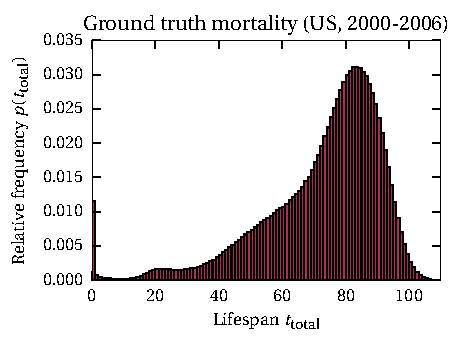
\includegraphics[width=0.49\textwidth]{media/mortality_ground_truth.pdf}
	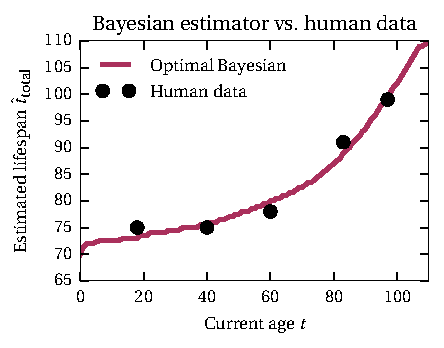
\includegraphics[width=0.49\textwidth]{media/mortality_optimal_bayesian_estimator.pdf}
	\caption{Ground truth mortality data $p(t_\mathrm{total})$ between the years 2000 and 2006 in the US (left), and the optimal Bayesian estimation for this data set (right). The human data collected by Griffiths et~al.~closely matches the optimal data. Ground truth data from the Human Mortality Database. University of California, Berkeley (USA), and Max Planck Institute for Demographic Research (Germany), available at \url{http://www.mortality.org/}, data downloaded 2017/03/27. Human data adapted from \cite{griffiths2006optimal}. The optimal prediction shown here is own work.}
	\label{fig:mortality_optimal}
\end{figure}
The hypothesis in the paper is that human predictions are optimal in the sense of a median estimator for the above model. If this hypothesis is true, the estimated $t_\mathrm{total}$ should correspond to the median of $p(t_\mathrm{total} \mid t)$. The median of a probability distribution $p(t_\mathrm{total} \mid t)$ is defined as the $t_\mathrm{total}$ for which
\begin{align}
	&\hphantom{=}
	   \;\; P(t_\mathrm{total} \leq \hat t_\mathrm{total} \mid t)
	 =  P(t_\mathrm{total} \geq \hat t_\mathrm{total} \mid t) \Leftrightarrow P(t_\mathrm{total} \leq \hat t_\mathrm{total} \mid t) - P(t_\mathrm{total} \geq \hat t_\mathrm{total} \mid t) = 0
	\label{eqn:median}
\end{align}
i.e.~it is equally likely for an actual $\hat t_\mathrm{total}$ to be either larger or smaller than the estimation. We can find optimal $\hat t_\mathrm{total}$ by solving (e.g.~numerically)
\begin{align}
	\begin{aligned}
	&\hphantom{=} P(t_\mathrm{total} \leq \hat t_\mathrm{total} \mid t) - P(t_\mathrm{total} \geq \hat t_\mathrm{total} \mid t) \\
	&=
		\int_{-\infty}^{\hat t_\mathrm{total}} \frac{p(t \mid t_\mathrm{total}) \cdot p(t_\mathrm{total})}{p(t)} \; \mathrm{d} t_\mathrm{total}
		-
		\int_{\hat t_\mathrm{total}}^{\infty} \frac{p(t \mid t_\mathrm{total}) \cdot p(t_\mathrm{total})}{p(t)} \; \mathrm{d} t_\mathrm{total}
		\\
	&=
		\int_{t}^{\hat t_\mathrm{total}} \frac{p(t_\mathrm{total})}{p(t) \cdot t_\mathrm{total}} \; \mathrm{d} t_\mathrm{total}
		-
		\int_{\hat t_\mathrm{total}}^{\infty} \frac{p(t_\mathrm{total})}{p(t) \cdot t_\mathrm{total}} \; \mathrm{d} t_\mathrm{total}
	\overset{!}= 0
	\,.
	\end{aligned}
	\label{eqn:optimal_inference}
\end{align}
Note that $p(t)$ is a constant scaling factor, which---as any other scaling factor---does not change the location of the zero-crossing.

Lifespan inference using this model is demonstrated in \cref{fig:mortality_optimal}. Human data collected by Griffiths et~al.~closely matches this optimal prediction, which suggests that humans must somehow be able to represent an equivalent of the above probability distributions and to draw conclusions from those. The next section outlines a simple mathematical framework for the representation of probability distributions and inference which, as I will demonstrate afterwards, can be used in a neural substrate.

\pagebreak
\section{Probability Distributions as Mixture Model}
\label{sec:pdist_mixture_model}

The lifespan inference task can be split into three steps: online learning of the prior distribution $p(t_\mathrm{total})$ from a set of samples $\hat t_\mathrm{total}$, calculation and representation of the conditional distribution $p(t_\mathrm{total} \mid t)$, and calculation of the median of the conditional distribution. In this section, I propose a very simple mixture model and discuss how it realizes each of the three required features.

\subsection{A non-negative mixture model for probability distribution learning}
\label{sec:mixture_model}

Our first goal is to learn the prior distribution $p(t_\mathrm{total})$, an online approximation of the empirical distribution $\mathfrak{P}(x)$ for $N$ samples $\hat X = \{\hat x_1, \ldots, \hat x_N\}$
\begin{align}
	\mathfrak{P}(x \mid \hat X) = \frac{1}N \cdot \sum_{i=1}^N \delta(x - \hat x_i) \,.
	\label{eqn:empirical_distr}
\end{align}
Generally, a probability distribution $p(x)$ is defined as a non-negative function $p(x) \geq 0$ normalized to one $\int_{-\infty}^{\infty} p(x) \,\mathrm{d}x = 1$. For a set of non-negative basis functions $\phi_i(x) \geq 0$, we can parameterize $p(x)$ as a mixture of $k$ basis functions
\begin{align}
	 p(x \mid \vec w) &= \frac{\sum_{i=1}^k w_i \cdot \phi_i(x)}{\sum_{i=1}^k w_i \cdot \int_{-\infty}^\infty \phi_i(x)} \,,
	 \label{eqn:mixture}
\end{align}
where $w_i > 0$ are non-negative weights. Depending on the choice of $\phi_i$, this representation is similar to Gaussian mixture models or, more general, Radial Basis Functions, which constrain $\phi_i$ to a function over the distance to a center point $\|x - x_i\|$ \cite{press2007numerical}.

To perform online learning, our goal is to find a weight vector $\vec w$ for which $p(x) \approx \mathfrak{P}(x \mid \hat X)$, one sample $\hat x_i$ at a time. A method commonly applied to probabilistic mixture models is Expectation Maximization (EM). Here, the calculation of the distribution parameters itself is treated as a statistical inference problem \cite{dempster1977maximum}. Since the basis functions $\phi_i$ in \cref{eqn:mixture} are non-parametric, the EM algorithm would collapse into a single E-step. Furthermore, while online versions of EM exist \cite{titterington1984recursive,cappe2009online}, we can use a far easier---and still optimal---weight update rule for the above mixture model.

For sake of simplicity, I ignore the probability density function normalization property, which, as any other scaling factor and as already hinted at in \cref{eqn:optimal_inference}, is irrelevant for Bayesian inference. From a frequentist point of view, a unnormalized $p(x)$ is the number of occurrences of $x$, equivalent to $\mathfrak{P}(x \mid \hat X) \cdot N$, \cref{eqn:empirical_distr}. I denote the unnormalized mixture model as
\begin{align}
	\mathfrak{p}(x \mid \vec w) &= \sum_{i=1}^k w_i \cdot \phi_i(x)\,.
	\label{eqn:mixture_denorm}
\end{align}
Ideally, whenever the system receives a sample $\hat x$, we want to update $\mathfrak{p}(x \mid \vec w)$ to
\begin{align}
	\mathfrak{p'}(x \mid \vec w') &= \mathfrak{p}(x \mid \vec w) + \delta(x - \hat x)\,.
\end{align}
In other words, $\mathfrak{p'}(x \mid \vec w')$ is increased by one exactly if $x = \hat x$ and unchanged for all $x \neq \hat x$. Given this ideal goal, we can calculate the optimal weight update $\Delta \vec w = \vec w' - \vec w$ by means of least squares error minimization
\begin{align}
	\begin{aligned}
	\frac{\mathrm{\partial}}{\mathrm{\partial}\Delta w_j} \; E &=
	\frac{\mathrm{\partial}}{\mathrm{\partial}\Delta w_j} \; \int_{-\infty}^\infty \frac{1}2
		\left(
			\mathfrak{p'}(x \mid \vec w') - \mathfrak{p}(x \mid \vec w) - \delta(x - \hat x) 
		\right)^2 \;\mathrm{d}x \\
	&= \frac{\mathrm{\partial}}{\mathrm{\partial}\Delta w_j} \; \int_{-\infty}^\infty \frac{1}2
		\left(
			\sum_{i=1}^k \Delta w_i \cdot \phi_i(x) - \delta(x - \hat x) 
		\right)^2 \;\mathrm{d}x \\
	&= \int_{-\infty}^\infty
			\sum_{i=1}^k \Delta w_i \cdot \phi_j(x) \cdot \phi_i(x) - \phi_j(x) \cdot \delta(x - \hat x) 
		\;\mathrm{d}x \\
	&= \sum_{i=1}^k \Delta w_i \cdot \underbrace{\int_{-\infty}^\infty \phi_j(x) \cdot \phi_i(x) \;\mathrm{d}x}_{\gamma_{ij}} - \phi_j(\hat x) \overset{!} = 0 \\
	\Leftrightarrow \Delta \vec w
	&= \Gamma^{-1} \cdot \vec \phi(\hat x) \,,
	\end{aligned}
	\label{eqn:update_rule}
\end{align}
where $\Gamma$ is a matrix of inner products $\gamma_{ij} = \langle \phi_i, \phi_j \rangle$. Note that this rule ignores the non-negativity of $\vec w$. Clamping of the weight vector to non-negative values is a possible solution, yet this increases the approximation error.

As a special case, consider orthogonal basis functions. It holds $\Gamma = I$ and correspondingly $\Delta \vec w = \vec \phi(\hat x)$. This means that $\Delta \vec w$ is just proportional to the value (activation) of the basis functions $\vec \phi$ and guarantees non-negative $\vec w$.

\subsection{Function space transformations: median calculation as gradient descent}

While I have not yet proposed how to represent the posterior conditional distribution needed for the lifespan inference task, I first would like show that we can perform a few interesting transformations of the functions space underlying the mixture model in \cref{eqn:mixture}, without changing the parameter vector $\vec w$ itself. As we will see in \cref{sec:architecture}, this is an important property required for the actual network implementation.

For example, we can calculate the cumulative distribution $P(x \leq \hat x)$ from $p(x)$ by just replacing the basis functions $\phi_i$ with their integral $\Phi_i'$
\begin{align}
	\begin{aligned}
    P(x \leq \hat x)
    &= \int_{-\infty}^{\hat{x}} p(x') \; \mathrm{d}x'
     = \int_{-\infty}^{\hat{x}} \sum_{i=1}^k w_i \cdot \phi_i(x) \; \mathrm{d}x' \\
    &= \sum_{i=1}^k w_i \cdot \underbrace{\int_{-\infty}^{\hat{x}} \phi_i(x') \;  \mathrm{d}x'}_{\Phi'_i(\hat x)}
     = \sum_{i=1}^k w_i \cdot \Phi'_i(\hat x) \,.
	\end{aligned}
    \label{eqn:cumulative_distribution}
\end{align}
This approach can easily be extended towards a strategy for the calculation of the median and can later be applied to the conditional probability distribution as well.

Remember that the difference between two the cumulative distributions in \cref{eqn:median} is zero exactly if $\hat x$ corresponds to the median. We can use this observation to calculate the median as gradient descent over time $t$:
\begin{align}
    \begin{aligned}
       -\frac{\mathrm{d} \hat x}{\mathrm{d}t}
    &= P(x \leq \hat x) - P(x \geq \hat x) \\
    &= \int_{-\infty}^{\hat{x}} p(x') \; \mathrm{d}x' - \int_{\hat{x}}^{\infty} p(x') \; \mathrm{d}x' \\
    &= \sum_{i=1}^k w_i \cdot \underbrace{\left(
        \int_{-\infty}^{\hat{x}} \phi(x') \; \mathrm{d}x' -
        \int_{\hat{x}}^{\infty} \phi(x') \; \mathrm{d}x'
       \right)}_{\Phi_i(\hat x)}
     = \sum_{i=1}^k w_i \cdot \Phi_i(\hat x) \,.
    \end{aligned}
    \label{eqn:median_dynamical}
\end{align}
Without providing a formal proof and only considering one-dimensional $x$, this dynamical system behaves as a line attractor for all $\hat x$ for which the median condition in \cref{eqn:median} is fulfilled. There are no other attractors in the system, since the probability density function $p(x)$ is non-negative, and correspondingly, the difference between the two cumulative distribution functions is monotone increasing. The system has a single stable attractor exactly if the cumulative function is strictly monotonic (i.e.~the probability density function $p(x)$ is positive).

\subsection{Representation of the conditional distribution}
\label{sec:conditional}

We can employ the same basis transformation technique shown above to compute conditional distributions. Given a fixed $p(y \mid x)$, it holds
\begin{align}
	p(x \mid y)
	&\propto p(y \mid x) \cdot p(x)
%	&=       p(y \mid x) \cdot \sum_i w_i \cdot \phi_i(x)
	 =       \sum_i w_i \cdot p(y \mid x) \cdot \phi_i(x)
	 =       \sum_i w_i \cdot \phi_i(x, y) \,.
	\label{eqn:conditional}
\end{align}
Correspondingly, all we have to do to calculate the conditional distribution for a learned $\vec w$ is to replace the original set of one-dimensional basis functions with a two dimensional set of basis functions. Of course, to calculate the median gradient we can still apply the results from \cref{eqn:median_dynamical} and obtain basis functions $\Phi_i(x, y)$:
\begin{align}
    \Phi_i(x, y) =
        \int_{-\infty}^{\hat{x}}
            p(y \mid x') \cdot \phi_i(x') \; \mathrm{d}x' -
        \int_{\hat{x}}^{\infty}
            p(y \mid x') \cdot \phi_i(x') \; \mathrm{d}x'
    \label{eqn:median_gradient_basis}
\end{align}


\subsection{Selecting radial basis functions}

\begin{figure}
	\centering
	\begin{subfigure}{0.37\textwidth}%
		\centering%
		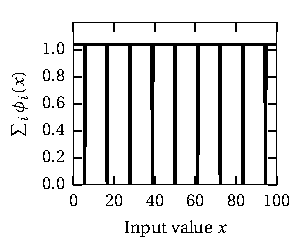
\includegraphics{media/basis_box.pdf}%
		\subcaption{Box basis}%
		\label{fig:basis_box}%
	\end{subfigure}%
	\begin{subfigure}{0.315\textwidth}%
		\centering%
		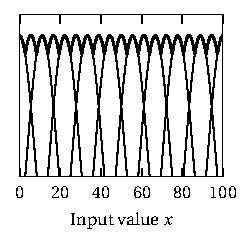
\includegraphics{media/basis_cosine.pdf}%
		\subcaption{Cosine basis}%
		\label{fig:basis_cosine}%
	\end{subfigure}%
	\begin{subfigure}{0.315\textwidth}%
		\centering%
		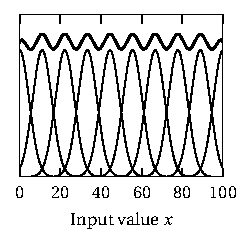
\includegraphics{media/basis_gaussian.pdf}%
		\subcaption{Gaussian basis}%
		\label{fig:basis_gaussian}%
	\end{subfigure}%
	\caption{Sketch of three possible sets of basis functions $\phi_i$ (thin lines) and their sum (thick line) for $k = 10$. Numerical instability in the parameter selection causes the box basis functions in (a) to be imperfectly aligned, causing the sum to become zero at times.}
	\label{fig:basis}
\end{figure}

Until now I have not defined the actual basis functions $\phi_i(x)$. In the following, I select $\phi_i$ as a set of radial basis functions \cite{press2007numerical}
\begin{align}
	\phi_i(x) = \phi\left(\frac{\| x - x_i \|}{\sigma}\right) \,,
	\label{eqn:rbf}
\end{align}
where $\sigma$ is a scale parameter for each radial basis $\phi(r)$. Note that I assume $\phi(0) = 1$, and $0 \leq \phi(r) \leq 1 \; \forall r$. The (one-dimensional) $x_i$ are uniformly distributed across the input domain. Basis functions of this kind are used in the convolution coding and gain encoding theories of probability density function representation presented in \cref{sec:introduction} \cite{knill2004bayesian,ma2006bayesian}. Possible choices for $\phi(r)$ include
\begin{align}
	  \phi^\mathrm{box}(r) &= \begin{cases}
				1 & \text{if } r \leq 1 \\
				0 & \text{if } r > 1
	           \end{cases},
	& \phi^\mathrm{cos}(r) &= \begin{cases}
	              \cos(r) & \text{if } r \leq \frac{\pi}2 \\
	              0       & \text{if } r > \frac{\pi}2 \\
	             \end{cases},
	& \phi^\mathrm{gauss}(r) &= \exp\left(-r^2\right) \;.
	\label{eqn:basis}
\end{align}

As pointed out above, the weight update rule in \cref{eqn:update_rule} can be simplified if $C \approx I$, which corresponds to the basis functions being orthogonal. It should be intuitively clear that two non-negative functions $\phi_i$, $\phi_j$ are orthogonal exactly if their product is zero
\begin{align}
	\langle \phi_i, \phi_j \rangle = \int_{-\infty}^\infty \phi_i(x) \cdot \phi_j(x) \;\mathrm{d}x = 0 \Leftrightarrow \phi_i(x) \cdot \phi_j(x) = 0 \;\forall x \;,
\end{align}
put differently, they are orthogonal, exactly if their non-zero values do not overlap. Thus, to achieve orthogonality, or at least near-orthogonality, $\sigma$ in \cref{eqn:rbf} must be chosen in such a way, that there is as little overlap between the bases as possible. Unfortunately, this condition runs contrary with ensuring that each point $x$ in the input domain is equally well represented by the basis. As a compromise, I choose $\sigma$ such that the following quadratic error
\begin{align}
	  E(\sigma) &= \left(1 - \min_x(f(x; \sigma))\right)^2 + \left(1 - \max_x(f(x; \sigma))\right)^2
	& \text{with } f(x; \sigma) &= \sum_{i = 1}^k \phi\left(\frac{\| x - x_i \|}{\sigma}\right)
\end{align}
is minimized. On the one hand, this minimizes overlap ($\phi(r) \approx 1$ for $|r| \approx 0$, large $\sigma$ would cause $f(x; \sigma) \gg 1$) and on the other hand makes sure that the support for each point $x$ (expressed by $f$) is approximately equivalent, since both the distance of the minimum and maximum value of $f$ from one are minimized.

\begin{figure}
	\centering%
	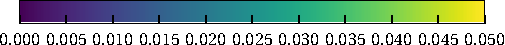
\includegraphics{media/inner_prod_cbar.pdf}\\[0.5cm]
	\begin{subfigure}{0.33\textwidth}%
		\centering%
		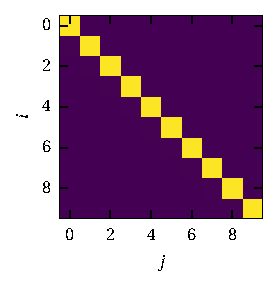
\includegraphics{media/basis_box_prod.pdf}%
		\caption{Box basis}%
	\end{subfigure}%
	\begin{subfigure}{0.33\textwidth}%
		\centering%
		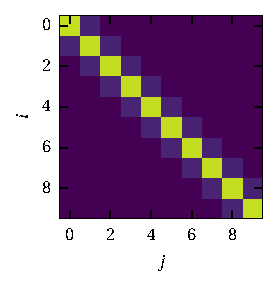
\includegraphics{media/basis_cosine_prod.pdf}%
		\caption{Cosine basis}%
	\end{subfigure}%
	\begin{subfigure}{0.33\textwidth}%
		\centering%
		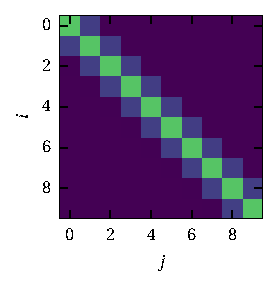
\includegraphics{media/basis_gaussian_prod.pdf}%
		\caption{Gaussian basis}%
	\end{subfigure}
	\caption{Visualization of the inner product matrices $\Gamma$ for the three basis function sets shown in \cref{fig:basis} with $k = 10$ basis functions. Each cell corresponds to the value of the matrix entry $\gamma_{ij}$.}
	\label{fig:basis_prod}
\end{figure}
An exemplary set of basis functions selected with the above method is shown in \cref{fig:basis} and the corresponding inner product matrices in \cref{fig:basis_prod}. The box basis functions do not overlap ($\Gamma = I$) and each point has exactly the same support. However, and in contrast to the cosine basis or the Gaussian basis, the box basis is not well representable in a neural substrate due to its discontinuities. The sum of Gaussian and cosine basis functions have considerable ripple, and there are some non-zero entries in the $\Gamma$ matrix off the main diagonal. For the cosine basis, the diagonal entries are approximately ten times larger than the diagonal entries, whereas for the Gaussian basis there is only a factor three difference. Nevertheless, $\Gamma \approx I$ seems quite reasonable in all cases.




\pagebreak
\section{Neurobiological Model}
\label{sec:architecture}

As discussed in \cref{sec:introduction}, there is strong evidence that nervous systems are capable of Bayesian inference. \emph{How} inference is implemented in a neural substrate is still an open debate. Correspondingly, any neural network implementation offers an hypothesis of how Bayesian inference could be implemented in the brain. Both performance and architecture of these models are predictions which must be compared to emerging psychophysical and neurobiological evidence.

To further constrain the model in terms of neurophysiology, it would be beneficial to know \emph{where} the implementation of Bayesian inference for the lifespan inference task is actually located in the brain. Unfortunately, most research concerning Bayesian inference focuses on low-level cognition, such as sensory processing, which (unsurprisingly) is theorized to be located in the cortical areas which process the corresponding sensory modality. For example, some neuroscientists argue---and provide evidence---that cortical visual pathways perform Bayesian inference by integrating contextual priors and observations through feedforward and feedback connections \cite{lee2003hierarchical}.

Even more discouraging is the fact that the lifespan inference task is a high-level cognitive task which involves subjects \emph{thinking} about the problem. Thus, the task is most likely distributed over various brain areas, including frontal cortex (state representation and working memory), the basal ganglia and striatum (action selection), and brain regions involved with long-term memory, such as hippocampus and the temporal cortex \cite{kandel2012principles}.

However, since the circuits underlying optimal Bayesian inference are probably similar for high- and low-level phenomena, and there is evidence that numbers are represented in prefrontal cortex and intraparietal sulcus \cite{nieder2009representation}, it seems reasonable to assume that the inference network is located somewhere on the frontal cortex. Correspondingly, the proposed neurobiological circuit for Bayesian inference has a simple feedforward architecture with control signals originating from other (not modeled) brain areas and a few recurrent connections required for median calculation over time.

\subsection{System description}

\begin{figure}[p]
    \centering
    \begin{subfigure}{\textwidth}%
        \centering%
        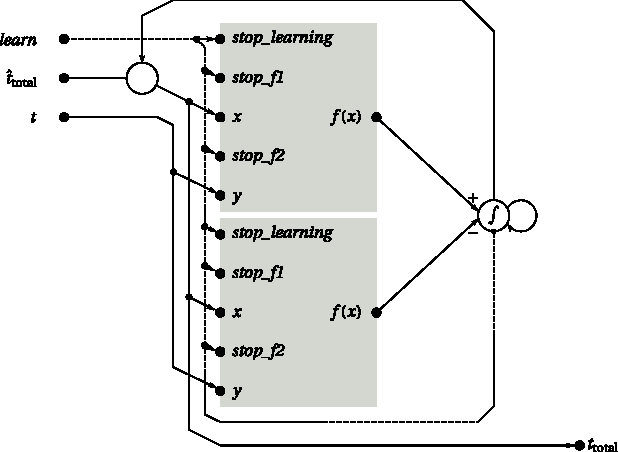
\includegraphics{media/diag_overall.pdf}%
        \caption{Overall system architecture}
        \label{fig:diag_overall}
    \end{subfigure}\\[1cm]
    \begin{subfigure}{\textwidth}%
        \centering%
        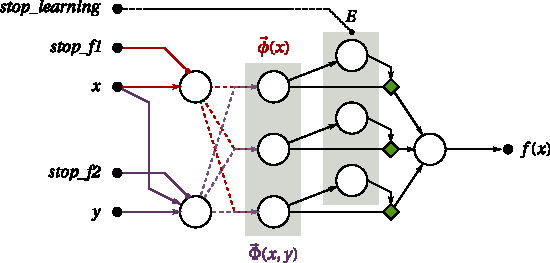
\includegraphics{media/diag_px.pdf}%
        \caption{Probability distribution network}
        \label{fig:diag_px}
    \end{subfigure}\\[1cm]
    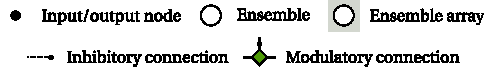
\includegraphics{media/diag_legend.pdf}\\[1cm]
    \caption{Architectural overview of the lifespan inference network. (a) The network is composed of two probability distribution networks computing the positive and negative branches of $\Phi(x, y)$ respectively. If the control input \emph{learn} is active, the network adapts its internal weights such that it represents the prior distribution sampled from $\hat t_\mathrm{total}$. If \emph{learn} is inactive, the network estimates a lifespan $t_\mathrm{total}$ given $t$ by integrating the median gradient function. (b) Probability distribution network with $k = 3$ basis functions. Switching between basis functions $\phi(x)$ and $\Phi(x, y)$ is performed by inhibiting the respective input populations using the \textit{stop\_f1} or \textit{stop\_f2} signals.}
    \label{fig:diag}
\end{figure}

The desired high-level behavior of the system is the lifespan inference task described in \cref{sec:lifespan_inference_task}. A corresponding high-level architectural overview of a network model is shown in \cref{fig:diag_overall}. The network model receives inputs $t$ and $\hat t_\mathrm{total}$, and produces an output $t_\mathrm{total}$. The input $t$ refers to the current age of a person $t$, $\hat t_\mathrm{total}$ is a ground-truth lifespan sample, and the output $t_\mathrm{total}$ corresponds to the median of the inferred distribution $p(t_\mathrm{total} \mid t)$.

For sake of simplicity, all values are scalar, real valued numbers in the range between 0 and 100. While in biology numbers might be encoded as (random) vectors in a high-dimensional space, neuroscientific data suggest that numbers (at least for small quantities) are both represented by both monotonic neurons, and cells tuned to specific quantities \cite{nieder2009representation}. The model is built upon the assumption that these can be decoded to a scalar value.

In addition to the above inputs, the network possesses a control input \emph{learn} which switches between the \emph{learning} and the \emph{inference} mode. In particular, $\hat t_\mathrm{total}$ should only influence the network in the \emph{learning} mode, while the opposite is true for $t$. Control signals perform feedforward inhibition on various ensembles in the network.

\paragraph{Probability distribution network}
The central component of the model is the probability distribution network sketched in \cref{fig:diag_px}. Note that the description of this component uses the abstract variable names from \cref{sec:mixture_model}. As a result of the learning mechanism elaborated below, the lifespan inference network requires two identical copies of this subcomponent, which calculate either the positive and or the negative branch of the median estimation basis functions $\Phi(x, y)$.

The subnetwork can compute two functions: the probability distribution $p(x)$ and the median gradient for the posterior distribution $p(x \mid y)$ as outlined in \cref{eqn:median_gradient_basis}. The input values for each of these functions are represented in different neuron ensembles. A one-dimensional ensemble represents $x$ and a two-dimensional ensemble represents $x$ and $y$ simultaneously. The individual basis functions $\phi_i(x)$ and $\Phi_i(x \mid y)$ are calculated in the connections between the input ensembles and a single, $k$-dimensional ensemble array representing $\vec \phi(x)$ or $\vec \Phi(x \mid y)$. The individual ensembles of this array additively project onto an output population, representing the final function value as defined in \cref{eqn:mixture_denorm}. Inhibiting one of the input ensembles allows to switch between the set of basis functions and thus the function being computed.

\paragraph{Learning mechanism}
The initial synaptic weights for the connections projecting from the basis function ensemble onto the output ensemble are set to zero. In order to adapt these weights and learn a probability distribution from sampling the input $x$, the original basis function set $\vec \phi(x)$ must be active. The activity of the central ensemble array representing $\vec \phi(x)$ is projected onto a similar ensemble array representing an error signal $E$. This error signal modulates the additive projections to the output node according to the prescribed error sensitivity (PES) rule proposed in \cite{macneil2011finetuning}
\begin{align}
    \Delta \vec d_i = \kappa \cdot E \cdot \vec a_i \,,
    \label{eqn:pes}
\end{align}
where $\vec d_i$ is the decoding vector, $\vec a_i$ is the pre-synaptic neural activity vector, $\kappa$ is the learning rate, and $E$ is the error signal. In the context of function learning, the error signal $E$ required to learn a function $f$ is the difference between the current function value $f(x)$ and the desired function value $\hat f(x)$. In the context of the probability distribution network, we would like to learn the function $\hat f(\phi_i(x)) = w'_i \cdot \phi_i(x)$, where $w_i'$ is our new, desired weight. Assume that the current function is $f(\phi_i(x)) = w_i \cdot \phi_i(x)$, where $w_i$ is an old weight from a previous step. A local error signal implementing the weight update derived in \cref{eqn:update_rule} is then given as
\begin{align}
	E_i &= f(\phi_i(x)) - \hat f(\phi_i(x))
		 = w_i \cdot \phi_i(x) - w'_i \cdot \phi_i(x)
		 = -\Delta w_i \cdot \phi_i(x)
		 = - (\Gamma^{-1} \cdot \vec \phi(x))_i \cdot \phi_i(x) \notag \\
		&\approx - (I \cdot \vec \phi(x))_i \cdot \phi_i(x) = -\phi_i(x)^2
		\,.
\end{align}
Consequently, the connection from the ensembles representing the basis function $\phi(x)$ to the error ensemble must calculate the negative square of the input. Weight adaptation can be interrupted by feedforward inhibition of the error signal ensembles.

This approach has a major drawback. The domain of the learned function $f$ is restricted to positive values, as the basis functions $\phi_i(x)$ are non-negative. Correspondingly, the PES rule in \cref{eqn:pes} will only adapt the decoders to account for positive values. When trying to compute the median gradient using the basis functions $\Phi_i(x, y)$ (which produce negative values), the learned connection from the basis function ensembles to the output population will strongly distort negative values. A solution to this problem is to split $\Phi_i(x, y)$ into two functions $\Phi^+_i(x, y)$ and $\Phi^-_i(x, y)$ computing the positive and the negative branch of the function separately as non-negative functions in separate probability distribution networks as shown in \cref{fig:diag_overall}.

\paragraph{Lifespan inference}
Given the probability distribution networks, implementing the actual lifespan inference is straight-forward. The \emph{learn} input disinhibits the error signal ensembles and the probability distribution basis functions $\phi_i(x)$. When switching to the inference mode, the median gradient function is disinhibited instead. The gradient produced by the two probability distribution networks is integrated and added to the current estimate $t_\mathrm{total}$, which is buffered in its own neural ensemble. Once the system stabilizes, the lifespan estimate $t_\mathrm{total}$ can be read from the network.

\paragraph{Neurobiological properties}
Typical pyramidal neurons in rat cortex have been found to have maximum steady firing rates of about $\SI{74}{\hertz}$ in vivo \cite{schwindt1997quantitative}, whereas in vitro the firing rates saturate at \SIrange{100}{300}{\hertz} \cite{mccormick1985comparative}. Fast-spiking inhibitory interneurons have been found to spike at much higher rates at much higher rates (\SIrange{500}{600}{\hertz}) \cite{azouz1997physiological}. Since the NEF model does not distinguish between excitatory and inhibitory neurons, I uniformly select maximum firing rates between 100 and \SI{200}{\hertz} as a compromise. Furthermore, all neurons have a membrane time constant of \SI{20}{\milli\second}, which is supported by physiological data for cortical pyramidal cells \cite{mccormick1985comparative}. The refractory period is set to \SI{2}{\milli\second}, which roughly corresponds to the inverse of the maximum in vitro firing rate \cite{mccormick1985comparative}. The synaptic time constant is set to \SI{5}{\milli\second}, roughly corresponding to those found in excitatory AMPA synapses and slow inhibitory GABA synapses \cite{azouz1997physiological,bartos2002fast}. An exception to this rule is the integrator ensemble, which uses an time constant of $\tau = \SI{100}{\milli\second}$ in its recurrent connection, which have been observed for NMDA synapses \cite{flint1997nr2a}.

\paragraph{Tuning curves}
Special care has been taken for the selection of tuning curves for neurons in the basis function and error ensemble arrays. Note that any neural activity (noise) in either ensemble causes potentially unwanted adaptions in the connection weights between the basis function ensembles and the output assemble as defined by the PES rule in \cref{eqn:pes}. The tuning curves are thus selected in such a way that a represented value of zero is encoded as zero neural activity. Since all represented values are non-negative (non-positive in the case of the error ensemble), this corresponds to sampling the $x$-intercepts for these neurons from $(0, 0.95)$ and setting encoders to one (minus one in the case of the error ensemble). For sake of simplicity, I use default uniform sampling with a radius of $100$ ($141$ in the case of the two-dimensional population) for all other ensembles. Note that this is not necessarily the best choice, since in most cases the value range from $-100$ to $100$ is not used in its entirety (i.e.~there are no negative ages).

\subsection{Design specification}

As already mentioned above, most ensembles represent ages between $0$ and $100$. For the inference task, it seems to be reasonable to expect a representation error of $10^{-3}$ for the variables $t$ and $t^\mathrm{total}$, which is theoretically achievable with less than $100$ neurons \cite{eliasmith2003neural}. To be on the safe side, and since I am using a lower maximum firing rate, I use $200$ neurons for all ensembles representing a one-dimensional age value, and $1000$ neurons for the two-dimensional populations representing both $t$ and $\hat t_\mathrm{total}$. This high neuron count is required, since the median gradient basis functions $\Phi(x, y)$ in \cref{eqn:median_gradient_basis} are rather complex. For two reasons, far fewer neurons are required for the representation of individual basis functions $\phi(x)$ and error values. First, I am only computing low-degree polynomials (a linear function and a square function) from these ensembles. Second, the represented values are integrated over time in either the weights or the output ensembles. Thus, the signal-to-noise ratio is not overly important. For a representation error of about one percent, we need about $20$ neurons for each basis function and error signal. However---and this is a major drawback of the proposed architecture---, care must be taken to exactly replicate the error and basis function ensembles in the two copies of the probability distribution network. If this is not ensured, slightly different weights will be learned, which distorts the median gradient function $\Phi(x, y)$.

The only dynamic component of the network is the integrator ensemble which integrates the median gradient. This ensemble is a one-dimensional working memory
\begin{align}
	\dot x &= x \Rightarrow A' = I, B' = \tau \,,
\end{align}
where $A'$ is the matrix describing the recurrent connection, $B'$ is the input transformation matrix, and $\tau$ is the recurrent synaptic time constant \cite{eliasmith2003neural}. Apart from these dynamics, there are no significant constraints regarding the timing of the network, e.g.~the Griffiths et~al.~paper neither reports any response times nor psychophysical timing.

\subsection{Implementation}

The actual implementation of the lifespan inference network is a direct translation of the above description into a Nengo \cite{bekolay2014nengo} model. As a decoding rule the default $L_2$ regression provided by Nengo is used. Evaluation points for decoding from the two-dimensional input population in the probability distribution network are sampled uniformly from the square $[0, 100] \times [0, 100]$. The probability distribution networks are modeled as reusable, separate subnetworks. Inputs $t$, $\hat t_\mathrm{total}$, $\mathit{learn}$ (and its negation) are generated in Python code and not simulated as neural networks. In particular, this is true for the inhibitory control signals in the probability distribution subnetwork. The two probability distribution networks are constructed using the same seeds for the individual error and basis function ensembles. This ensures that both networks learn exactly the same weights $w_i$.

\pagebreak
\section{Experiments}
\label{sec:experiments}

In this section I describe two sets of experiments. First, I analyze the accuracy of the probability distribution learning network for the box, rectified cosine and Gaussian basis function types introduced in \cref{eqn:basis} and depicted in \cref{fig:basis}, while varying the number of basis functions $k$. Second, I test the lifespan inference network as a whole and compare its predictions to both mathematically optimal results and the human performance data shown in \cref{fig:mortality_optimal}.

\subsection{Probability distribution network analysis}

\begin{sidewaysfigure}
	\centering
	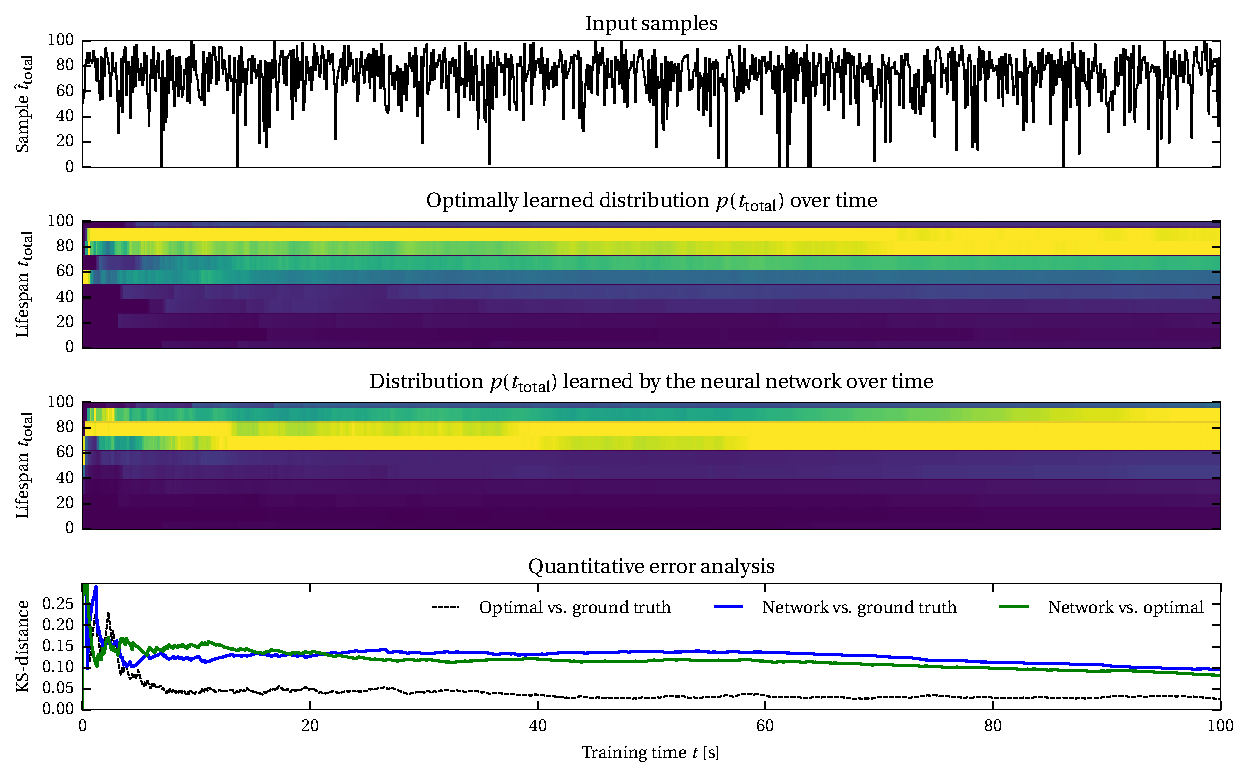
\includegraphics{media/net_probability_box_10_100000_0.pdf}
	\caption{Probability distribution learning experiment for a box basis with $k = 10$ bases. The probability distribution over time plots are scaled such that yellow corresponds to the maximum value in each time-slice. Darker colours correspond to smaller values.}
	\label{fig:analysis_pdist_box}
\end{sidewaysfigure}
\begin{sidewaysfigure}
    \centering
    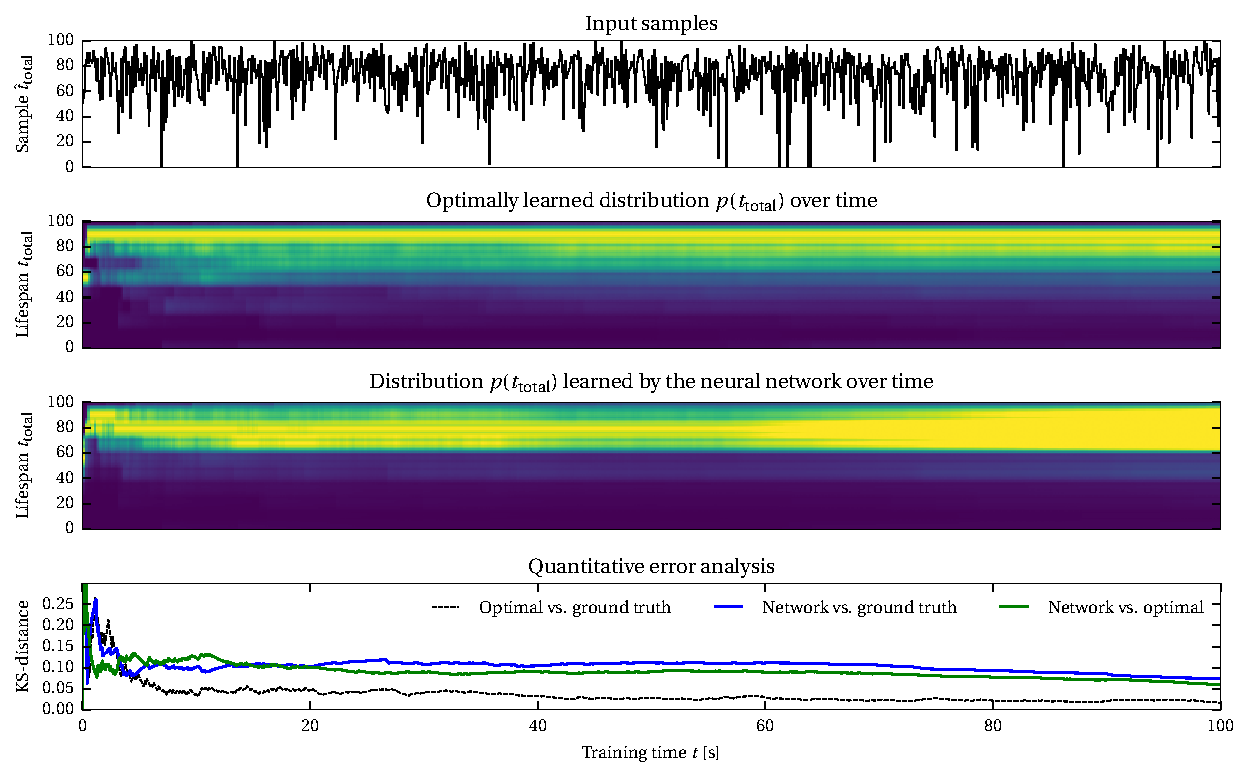
\includegraphics{media/net_probability_cosine_10_100000_0.pdf}
    \caption{Probability distribution learning experiment for a rectified cosine basis with $k = 10$. The probability distribution over time plots are scaled such that yellow corresponds to the maximum value in each time-slice. Darker colours correspond to smaller values.}
    \label{fig:analysis_pdist_cos}
\end{sidewaysfigure}
\begin{sidewaysfigure}
    \centering
    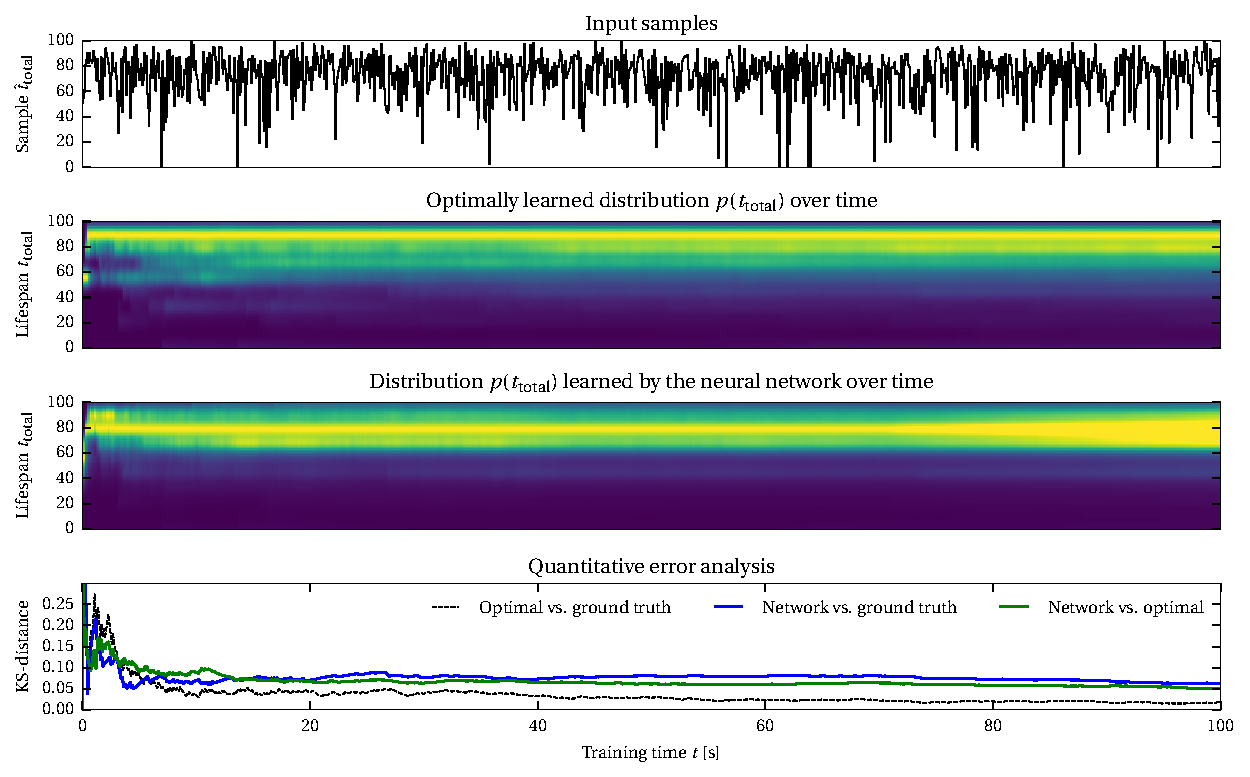
\includegraphics{media/net_probability_gaussian_10_100000_0.pdf}
    \caption{Probability distribution learning experiment for a Gaussian basis with $k = 10$. The probability distribution over time plots are scaled such that yellow corresponds to the maximum value in each time-slice. Darker colours correspond to smaller values.}
    \label{fig:analysis_pdist_gauss}
\end{sidewaysfigure}
\begin{figure}
	\centering%
 	\begin{subfigure}{0.33\textwidth}%
		\centering%
		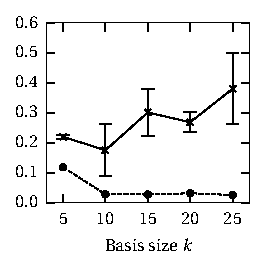
\includegraphics{media/net_probability_box_errs.pdf}%
		\subcaption{Box basis}%
	\end{subfigure}%
	\begin{subfigure}{0.33\textwidth}%
		\centering%
		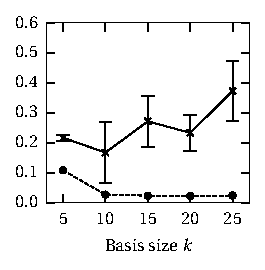
\includegraphics{media/net_probability_cosine_errs.pdf}%
		\subcaption{Cosine basis}%
	\end{subfigure}%
	\begin{subfigure}{0.33\textwidth}%
		\centering%
		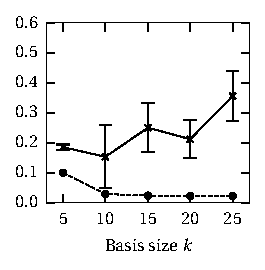
\includegraphics{media/net_probability_gaussian_errs.pdf}%
		\subcaption{Gaussian basis}%
	\end{subfigure}%
	\caption{Mean representation error (two-sample Kolmogorov-Smirnov metric) after \SI{50}{\second} of training for varying basis function counts $k$. Error bars indicate the standard deviation. Dashed lines corresponds to the optimally learned distribution. Data were gathered over five trials (each with a different network seed and samples) and the last 10\% of samples for each trial.}
	\label{fig:net_probability_errs}
\end{figure}


\paragraph{Method}
In the following experiments, I train a single probability distribution network by sampling from the ground truth lifespan distribution (\cref{fig:mortality_optimal}). Each sample $\hat t_\mathrm{total}$ is presented for \SI{100}{\milli\second} to the $x$-input of the probability distribution network (\cref{fig:diag_px}). To analyze the represented probability distribution while training progresses, I record the decoding vectors $\vec d_i(t)$ from the connections between the basis function ensemble $i$ and the output ensemble in \SI{10}{\milli\second} time slices. I reconstruct the mixture weights $w_i$ in \cref{eqn:mixture_denorm} by fitting a straight line to the decoded function
\begin{align}
    \langle \vec a_i(x),  \vec d_i(t) \rangle \overset{!}\approx w_i(t) \cdot x \,\forall x \in [0, 1]\,,
\end{align}
where $\vec a_i(x)$ corresponds to the basis function ensemble tuning curves. The resulting weight vector $\vec w(t)$ fully describes the probability distribution $p(t_\mathrm{total})$ represented by the network at time $t$. Note that---in contrast to the post-synaptic activity in the output ensemble, which is not evaluated here---the decoders do not saturate. I therefore artificially clamp the the learned probability distribution $p(t_\mathrm{total})$ to the interval $[0, 1]$ for evaluation purposes. The learning rate for the PES rule in \cref{eqn:pes} is fixed to $\kappa = 2\cdot10^{-5}$.

As an evaluation measure, I compare the learned probability distribution to optimally learned weights (\cref{eqn:update_rule}, no clamping applied here) and the ground truth distribution. Furthermore, to obtain a baseline performance for the selected basis function type and count, I compare the optimally learned probability distribution to the ground truth. I use the two-sample Kolmogorov-Smirnov statistic \cite{massey1951kolmogorov} as a dissimilarity metric (and not a s a statistical test) for two one-dimensional probability distributions $p(x)$, $q(x)$
\begin{align}
    D^\mathrm{KS}(p, q) = \max_x
        \left| \int_{-\infty}^x p(x') \, \mathrm{d}x' - \int_{-\infty}^x q(x') \,\mathrm{d}x' \right| \,.
	\label{eqn:dks}
\end{align}
In terms of a dissimilarity metric, it holds $D^\mathrm{KS}(p, q) = 0$ exactly if $p = q$, and $D^\mathrm{KS}(p, q) = 1$ exactly if $p$ and $q$ are orthogonal.


\paragraph{Results}
Figures \cref{fig:analysis_pdist_box,fig:analysis_pdist_cos,fig:analysis_pdist_gauss} visualize the probability distribution learning process for the optimal weight update and the neural network model over a \SI{100}{\second} training period. Individual figures show different basis function types, while the number of basis functions is $k = 10$. This results in a network of $800$ neurons (400 for the input and output populations, 400 for the basis and error signal ensembles). In all cases, the representation error steadily decreases over time. Regardless of the basis function type, the optimally learned distribution converges to an error of approximately $0.02$ compared to the ground truth distribution. This is not true for the representation error of the probability distribution represented by the neural network. For the box basis, the final representation error compared to ground truth is $0.095$, for the rectified cosine basis the error is $0.074$, and for the Gaussian basis the error is  $0.062$. Furthermore, saturation effects are clearly visible for the box and cosine basis starting at about $t = \SI{60}{\second}$, whereas the first signs of saturation are visible a little later at $t = \SI{70}{\second}$ in conjunction with the Gaussian. Overall, a relatively small representation error is reached after a timespan of about $\SI{20}{\second}$.

An interesting artifact in comparison to the optimally learned weights is that the neural implementation seems to shift the distribution towards younger ages. For example, for optimal weights the maximum of $p(t_\mathrm{total})$ is located at about $90$, whereas it is located at $80$ in all network simulations.

\Cref{fig:net_probability_errs} depicts the representation error after \SI{50}{\second} of training for basis function counts ranging from $k = 5$ to $k = 25$. Qualitatively, the choice of the basis function type has little impact on the shape of the curve. While the representation error of the optimally learned probability distribution stabilizes at a relatively small error for $k = 10$ onward, the neural network performance decreases for larger $k$. Additionally, the standard deviation is relatively large when testing different networks and sets of samples.

\paragraph{Discussion}
The results clearly show that the network is capable of learning the prior distribution $p(t_\mathrm{total})$ at a relatively small error level. While the basis function type had a significant impact on the representation error in the first part of the experiment, these differences turn out to be relatively small when performing repeating trials yet nevertheless are still visible. The increasing error for larger $k$ may be explained by the fact that it becomes more difficult to properly decode the basis functions from the input ensemble. For increasing $k$, the basis functions are slimmer, converging to a Dirac-$\delta$, and thus require higher frequencies in the function space spanned by the input ensemble. Faster and slower saturation depending on the basis function type in the first part of the experiment is simply caused by the area under the individual basis functions being different, and thus $\phi_i(x)$ being larger for the box and cosine bases.

\subsection{Lifespan inference experiments}

\begin{sidewaysfigure}
	\centering
	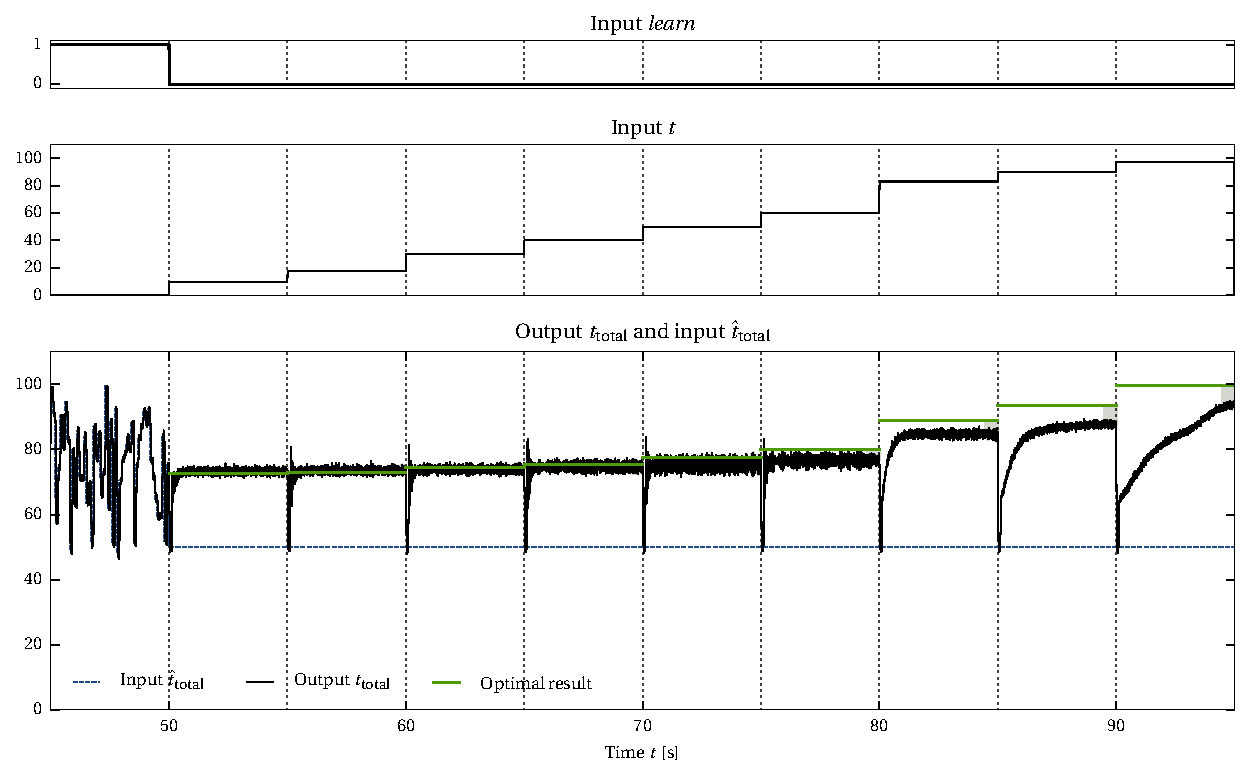
\includegraphics{media/net_lifespan_gaussian_10_const_0.pdf}
	\caption{Input and output values of the lifespan inference network over time. A constant initial value $\hat t_\mathrm{total}$ is used. Shaded gray areas in the bottom plot correspond to the regions included in the error analysis.}
	\label{fig:net_lifespan_const}
\end{sidewaysfigure}
\begin{sidewaysfigure}
	\centering
	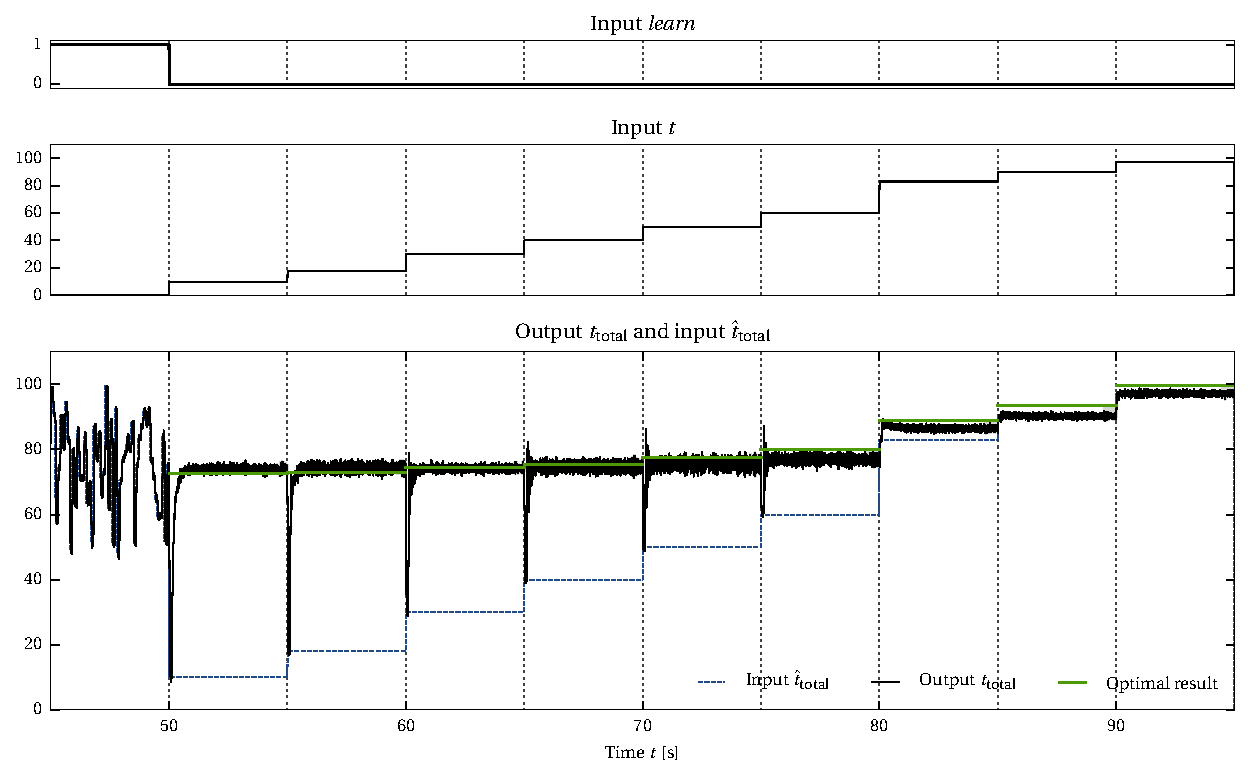
\includegraphics{media/net_lifespan_gaussian_10_t_0.pdf}
	\caption{Input and output values of the lifespan inference network over time. The initial value $\hat t_\mathrm{total}$ is set to the input $t$. Shaded gray areas in the bottom plot correspond to the regions included in the error analysis.}
	\label{fig:net_lifespan_t}
\end{sidewaysfigure}
\begin{figure}
	\centering%
	
\includegraphics{media/net_lifespan_analysis_legend.pdf}\\[0.25cm]%
	\begin{subfigure}{0.5\textwidth}%
		\centering
		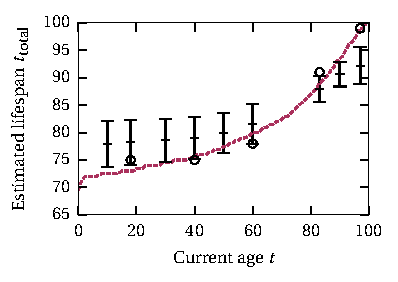
\includegraphics{media/net_lifespan_gaussian_10_const_analysis.pdf}%
		\caption{Constant initial value $\hat t_\mathrm{total}$}%
	\end{subfigure}%
	\begin{subfigure}{0.5\textwidth}%
		\centering%
		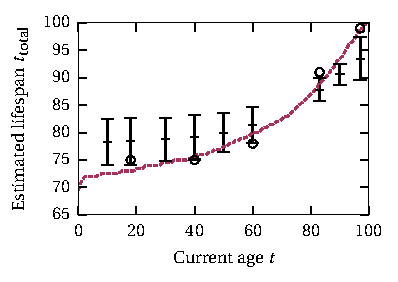
\includegraphics{media/net_lifespan_gaussian_10_t_analysis.pdf}%
		\caption{Initial value $\hat t_\mathrm{total} = t$}%
	\end{subfigure}%
	\caption{Comparison between the inference performed by the network and both optimal and human data. Depicted network responses are means over 10 different networks. Error bars show the standard deviation.}
	\label{fig:net_lifespan_analysis}
\end{figure}

\paragraph{Method}
Evaluation of the lifespan inference network is divided into two phases: training and testing. The training phase has a total duration of \SI{50}{\second} and follows the procedure already employed for the analysis of the probability distribution network. During training, the $\mathit{learn}$ input is set to one, and samples $\hat t_\mathrm{total}$ are drawn from the ground truth distribution. Each sample is presented to the network for \SI{100}{\milli\second}.

For the evaluation phase, the $\mathit{learn}$ input is set to zero. Inferred lifespans $t_\mathrm{total}$ are queried by presenting ages to the input $t$ and waiting for \SI{5}{\second} for the network to settle. Presented ages include the values tested by Griffiths et~al. Note that in inference mode the input $\hat t_\mathrm{total}$ acts as an initial value for gradient descent. It is either set to a constant value or, in a second experiment, to the input $t$ itself. For the error analysis, the estimated $t_\mathrm{total}$ is filtered with a synaptic low-pass filter with $\tau = \SI{20}{\milli\second}$. Data from the last $10\%$ of the presentation period is used to calculate the average response and standard deviation. To ensure independence between the individual queries, the integrator ensemble is reset with a \SI{100}{\milli\second} inhibitory pulse at the beginning of each query. $k = 10$ Gaussian basis functions are used for the prior probability distribution, resulting in a total of $4000$ neurons.

\paragraph{Results}
Input and output values of the inference network over time are shown in \cref{fig:net_lifespan_const,fig:net_lifespan_t}. For small input values $t$, the network response quickly (within a new hundred milliseconds) converges towards the optimal value. In a few cases, the response overshoots, but quickly returns to smaller values. Significant noise is visible in most of the responses.

Interestingly, and as visible in the plot for a constant initial value $\hat t_\mathrm{total}$ \cref{fig:net_lifespan_const}, convergence is significantly slower for large $t$. In some instances the network even settles at lifespans $t_\mathrm{total}$ below the current age of the person, which is mildly unsettling. In the particular experiment runs shown here, this problem does not occur if $t$ is used as initial value for the median estimation. However, in some experiments the estimate actually converges back to values smaller than $t$.

A comparison between the network response, optimal Bayesian inference and human data is given in \cref{fig:net_lifespan_analysis}. The network response is not as good as the human data. Most of the times, inferred lifespans are too large for small $t$ and too small for large $t$. Significant variance in the response produced by different network instances is visible. Overall, the choice of the initial value does not exorbitantly influence the results.

\paragraph{Discussion}
Given that the network learned the underlying prior distributions in a short time and from few samples, the results are surprisingly good. They demonstrate that the presented framework for probability distribution representation and statistical inference can in fact be implemented as a spiking neural network.

Part of the variance in the inferred lifespans is caused by the noise in the output $t_\mathrm{total}$, which mostly consists of unwanted oscillations in the integrator ensemble. Slower integration time constants will probably resolve this issue, yet will result in slower convergence. Slow convergence for large $t$ can be explained with a small median gradient produced by the probability distribution networks. At some point, this gradient is below the noise floor, causing the integrator to stop at small $t_\mathrm{total}$. Too large responses for smaller $t$ may either be caused by the prior distribution being incorrectly represented, or distortion of the median gradient basis functions. The first suggestion seems unlikely since (as reported in the previous experiment), the prior distribution seems shifted towards shorter lifespans.

\pagebreak
\section{Conclusion}
\label{sec:conclusion}

In this report I presented a simple neurobiological architecture capable of learning a prior distribution and performing Bayesian inference by estimating the median of the posterior distribution. Experiments show that learning the prior lifespan distribution $p(t_\mathrm{total})$ with relatively small error is indeed possible with a network of about $800$ neurons. Likewise, the inference task itself works surprisingly well with mild deviations compared to the optimal model.

Undoubtedly, the presented model has several strength. Learning is expressed in terms of a local update rule. The error signal only depends on the activity of the pre-synaptic neuron population. Furthermore, the model mostly consists of feedforward connectivity with trivial, biologically plausible functions being computed between most populations. The proposed architecture requires relatively few neurons, with only $4000$ neurons for the entire lifespan inference tasks, which roughly corresponds to \SI{0.04}{\square\milli\meter} of cortical area \cite{carlo2013structural}.

Equally undoubted is the fact that the model has a large number of drawbacks compared to other approaches. A central weakness of the model is the need for two probability distribution representation networks to compute both the positive and the negative branch of the median gradient basis $\Phi(x, y)$. Additionally, the represented probability distributions are not normalized while learning, resulting in saturation of the output ensemble as learning progresses. In contrast to pure feedforward architectures, the recurrent median estimation is relatively slow, requiring up to \SI{5}{\second} for the network to settle on an output value.  The requirement for both positive and approximately orthogonal basis functions essentially restricts potential bases to bell-shaped curves, which inevitably resemble Dirac-$\delta$ functions for large bases. While technically orthogonality is not a strict requirement, non-orthogonal basis functions would cause the learning rule to be non-local, since $\Gamma \neq I$ in \cref{eqn:update_rule}. Another weakness of the model is that individual parts of the network have to be inhibited in order to switch between a \enquote{learning} mode and a \enquote{inference} mode. Simultaneous inference and training is not possible.

Future work should try to address the above weaknesses. Additionally, more detailed experiments such as training other prior probability distributions or varying neuron counts should be performed. Significant improvements in performance and resource utilization may be possible with some low-hanging fruits in the model implementation, such as better basis function decoding by concentrating the tuning-curve $x$-intercepts in the relevant ranges and by merging ensembles duplicated in the two probability distribution networks (input representations, error signal, output ensemble).

% Possible shortcomings
% - Requires symetric network for positive/negative branch
% - No normalization of the learned distribution
% - Wasteful basis functions (though basis function selection is not really limited)
% - Requires quite some time to converge to a solution
% - Individual parts of the network have to be switched on/off depending on wether to learn
%   or to perform inference

% Future work
% - Test for other distributions

\pagebreak
\printbibliography

\end{document}
